\documentclass[11pt]{article}
\usepackage{header}
\def\title{HW 04}

\begin{document}
\maketitle
\fontsize{12}{15}\selectfont

\begin{center}
    Due: Saturday, 9/23, 4:00 PM \\
    Grace period until Saturday, 9/23, 6:00 PM \\
\end{center}

\section*{Sundry}
Before you start writing your final homework submission, state briefly how you worked on it.  Who else did you work with?  List names and email addresses.  (In case of homework party, you can just describe the group.)

\vspace{15pt}

\Question{Modular Practice}

\notelinks{\href{https://www.eecs70.org/assets/pdf/notes/n6.pdf}{Note 6}}
Solve the following modular arithmetic equations for $x$ and $y$.
\begin{Parts}
\Part $9x+5 \equiv 7 \pmod{13}$.

\Part Show that $3x+12 \equiv 4 \pmod{21}$ does not have a solution.

\Part The system of simultaneous equations
$5x+4y \equiv 0 \pmod{7}$ and $2x+y \equiv 4 \pmod{7}$.

\Part $13^{2023} \equiv x \pmod{12}$.

\Part $7^{62} \equiv x \pmod{11}$.

\end{Parts}

\Question{Nontrivial Modular Solutions}

\notelinks*{\href{https://www.eecs70.org/assets/pdf/notes/n6.pdf}{Note 6}}
\begin{Parts}
    \Part What are all the possible perfect cubes modulo 7? In other words, compute the set
    \[
        \{x^3 \bmod{7} \mid x \in \mathbb{Z}\}
    .\]

    \Part Show that any solution to $x^3 + 2y^3 \equiv 0 \pmod{7}$ must satisfy $x \equiv y \equiv 0 \pmod{7}$.

    \Part Using part (b), prove that $x^3 + 2y^3 = 7x^2 y$ has no non-trivial solutions $(x, y)$ in the integers. In other words, there are no integers $x$ and $y$, that satisfy this equation, except the trivial solution $x=y=0$.

    [\emph{Hint:} Consider some nontrivial solution $(x, y)$ with the smallest value for $\abs{x}$ (why are we allowed to consider this?). Then arrive at a contradiction by finding another solution $(x', y')$ with $\abs{x'} < \abs{x}$.]

\end{Parts}

\Question{Squares}

\notelinks{\href{https://www.eecs70.org/assets/pdf/notes/n6.pdf}{Note 6},\href{https://www.eecs70.org/assets/pdf/notes/n7.pdf}{Note 7}}
Let $p$ be a prime greater than 2. We will prove that there exists an integer $a$ such that $a^2 \equiv -1 \pmod{p}$ if and only if $p \equiv 1 \pmod{4}$.

\begin{Parts}
	\Part Show that if $p \equiv 3 \pmod{4}$, there is no integer $a$ such that $a^2 \equiv -1 \pmod{p}$. (Hint: Use Fermat's Little Theorem.)

    \Part Wilson's Theorem states the following is true if and only if $p$ is prime:
    \[(p - 1)! \equiv -1 \pmod{p}.\]
    Prove both directions (it holds if \emph{and} only if $p$ is prime).

    Hint for the if direction: Consider rearranging the terms in $(p - 1)! = 1 \cdot 2 \cdot \cdots \cdot (p - 1)$ to pair up terms with their inverses, when possible. What terms are left unpaired?

    Hint for the only if direction: If $p$ is composite, then it has some prime factor $q$.  What can we say about $(p-1)! \pmod{q}$?

    \Part Show that if $p \equiv 1 \pmod{4}$, there is an integer $a$ such that $a^2 \equiv -1 \pmod{p}$. (Hint: Consider $a = \left(\frac{p - 1}{2}\right)!$, then use Wilson's Theorem.)
\end{Parts}

\Question{Celebrate and Remember Textiles}
\notelinks{\href{https://www.eecs70.org/assets/pdf/notes/n6.pdf}{Note 6}}
Mathematics and computing both owe an immense debt to textiles, where many key ideas originated.

Instructions for knitting patterns will tell you to begin by ``casting
on'' the needle some multiple of $m$ plus $r$, where $m$ is the number
of stitches to create one repetition of the pattern and $r$ is the
number of stitches needed for the two edges of the piece. For example,
in the simple rib stitch pattern below, the repeating pattern is of
length $m=4$, and you need $r=2$ stitches for the edges.
\begin{center}
    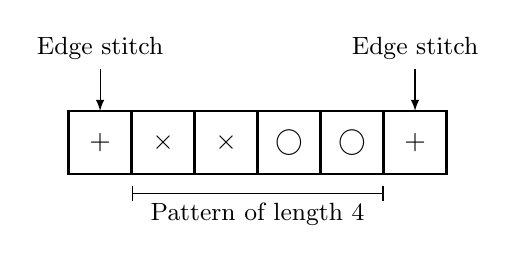
\begin{tikzpicture}[>=latex]
        \def\scale{0.8}
        \foreach[count=\x from 0] \val in {+,\times,\times,\bigcirc,\bigcirc,+} {
            \draw[thick] ({\scale*\x}, 0) rectangle ({\scale*\x+\scale}, \scale);
            \node[thick] at ({\scale*\x+0.5*\scale}, {0.5*\scale}) {$\val$};
        }
        \draw[Bar-Bar] (\scale, -0.25) -- (5*\scale, -0.25) node[below, pos=0.5] {\small Pattern of length 4};
        \node (edge-1) at (0.5*\scale, 2*\scale) {\small Edge stitch};
        \draw (edge-1) edge[->] (0.5*\scale, \scale);
        \node (edge-2) at (5.5*\scale, 2*\scale) {\small Edge stitch};
        \draw (edge-2) edge[->] (5.5*\scale, \scale);
    \end{tikzpicture}
\end{center}
Thus, to make the final piece wider, you can add as many multiples of the pattern of length 4 as you like;
for example, if you want to repeat the pattern 3 times, you need to cast on a total of $3m+ r = 3(4) + 2 = 14$ stitches (shown below).
\begin{center}
    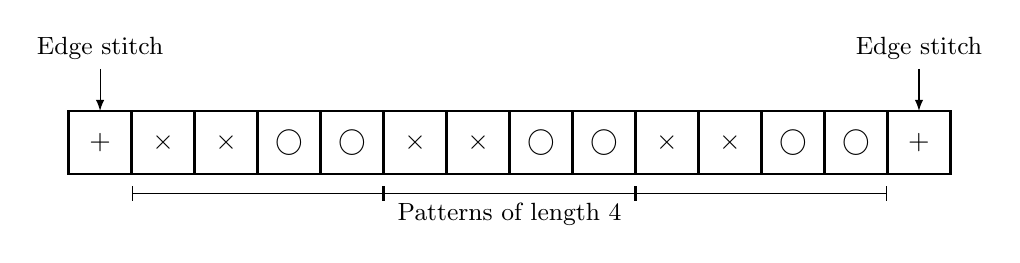
\begin{tikzpicture}[>=latex]
        \def\scale{0.8}
        \foreach[count=\x from 0] \val in {+,\times,\times,\bigcirc,\bigcirc,\times,\times,\bigcirc,\bigcirc,\times,\times,\bigcirc,\bigcirc,+} {
            \draw[thick] ({\scale*\x}, 0) rectangle ({\scale*\x+\scale}, \scale);
            \node[thick] at ({\scale*\x+0.5*\scale}, {0.5*\scale}) {$\val$};
        }
        \draw[Bar-Bar] (\scale, -0.25) -- (5*\scale, -0.25);
        \draw[Bar-Bar] (5*\scale, -0.25) -- (9*\scale, -0.25) node[below, pos=0.5] {\small Patterns of length 4};
        \draw[Bar-Bar] (9*\scale, -0.25) -- (13*\scale, -0.25);

        \node (edge-1) at (0.5*\scale, 2*\scale) {\small Edge stitch};
        \draw (edge-1) edge[->] (0.5*\scale, \scale);
        \node (edge-2) at (13.5*\scale, 2*\scale) {\small Edge stitch};
        \draw (edge-2) edge[->] (13.5*\scale, \scale);
    \end{tikzpicture}
\end{center}
You've decided to knit a 70-themed baby blanket as a gift for your cousin and
want to incorporate rows from three different stitch patterns with the
following requirements:
\begin{itemize}
\item Alternating Link: Multiple of 7, plus 4
\item Double Broken Rib: Multiple of 4, plus 2
\item Swag: Multiple of 5, plus 2
\end{itemize}

You want to be able to switch between knitting these different
patterns without changing the number of stitches on the needle, so you
must use a number of stitches that simultaneously meets the requirements of all three
patterns.

Find the \emph{smallest number of stitches} you need to cast on in
order to incorporate all three patterns in your baby blanket.

\Question{Euler's Totient Theorem}

\notelinks{\href{https://www.eecs70.org/assets/pdf/notes/n6.pdf}{Note 6},\href{https://www.eecs70.org/assets/pdf/notes/n7.pdf}{Note 7}}
Euler's Totient Theorem states that, if $n$ and $a$ are coprime,
\[
  a^{\phi(n)} \equiv 1 \pmod{n}
\]
where $\phi(n)$ (known as Euler's Totient Function) is the number of positive
integers less than or equal to $n$ which are coprime to $n$ (including 1).

\begin{Parts}
  \Part Let the numbers less than $n$ which are coprime to $n$ be $m_1, m_2, \ldots, m_{\phi(n)}$. 
  Argue that the set
  \[\{am_1, am_2, \ldots, am_{\phi(n)}\}\]
  is a permutation of the set
  \[\{m_1, m_2, \ldots, m_{\phi(n)}\}.\]
  In other words, prove that 
  \[f:\{m_1, m_2, \ldots, m_{\phi(n)}\} \to \{m_1, m_2, \ldots, m_{\phi(n)}\}\]
  is a bijection, where $f(x) \coloneqq ax \pmod{n}$.

  \Part Prove Euler's Theorem. (Hint: Recall the FLT proof.)
\end{Parts}

\Question{Sparsity of Primes}

\notelinks{\href{https://www.eecs70.org/assets/pdf/notes/n6.pdf}{Note 6}}
A prime power is a number that can be written as $p^i$ for some prime $p$ and some
positive integer $i$. So, $9 = 3^2$ is a prime power, and so is $8 = 2^3$. $42 = 2 \cdot 3 \cdot 7$ is not
a prime power.

Prove that for any positive integer $k$, there exists $k$ consecutive positive integers
such that none of them are prime powers.

\emph{Hint: This is a Chinese Remainder Theorem problem. We want to find $n$ such that $(n + 1)$, $(n + 2)$, \ldots, and $(n + k)$ are all not powers of primes. We can enforce this by saying that $n + 1$ through $n + k$ each must have two distinct prime divisors.}

\end{document}
